\begin{frame}
\frametitle{Handling varying degrees of multiplexing}
\begin{table}
\begin{center}
\begin{scriptsize}
\begin{tabular}{l|l|l|l|l|l}
\bf RemyCC & \bf Link speeds & \bf On avg. & \bf Off avg. & \bf min-RTT &
\bf \# senders \\
\hline
1--2     & 15 Mbps & 1 sec & 1 sec & 150 ms & 2 \\
1--10    & 15 Mbps & 1 sec & 1 sec & 150 ms & 10 \\
1--20    & 15 Mbps & 1 sec & 1 sec & 150 ms & 20 \\
1--50    & 15 Mbps & 1 sec & 1 sec & 150 ms & 50 \\
1--100   & 15 Mbps & 1 sec & 1 sec & 150 ms & 100 \\
\end{tabular}
\end{scriptsize}
\caption{Training scenarios for breadth in multiplexing}
\label{table:multiplexing}
\end{center}
\end{table}

\begin{table}
\begin{center}
\begin{scriptsize}
\begin{tabular}{l|l|l|l|l|l}
\bf Link speeds & \bf On avg. & \bf Off avg. & \bf min-RTT &
\bf \# senders & Buffer \\
\hline
15 Mbps & 1 sec & 1 sec & 150 ms & 1--100 & 5 BDP\\
\end{tabular}
\end{scriptsize}
\caption{Testing scenarios for breadth in multiplexing}
\label{table:muxtesting}
\end{center}
\end{table}

\end{frame}

\begin{frame}
\frametitle{Handling varying degrees of multiplexing}
\begin{centering}

\noindent \only<1>{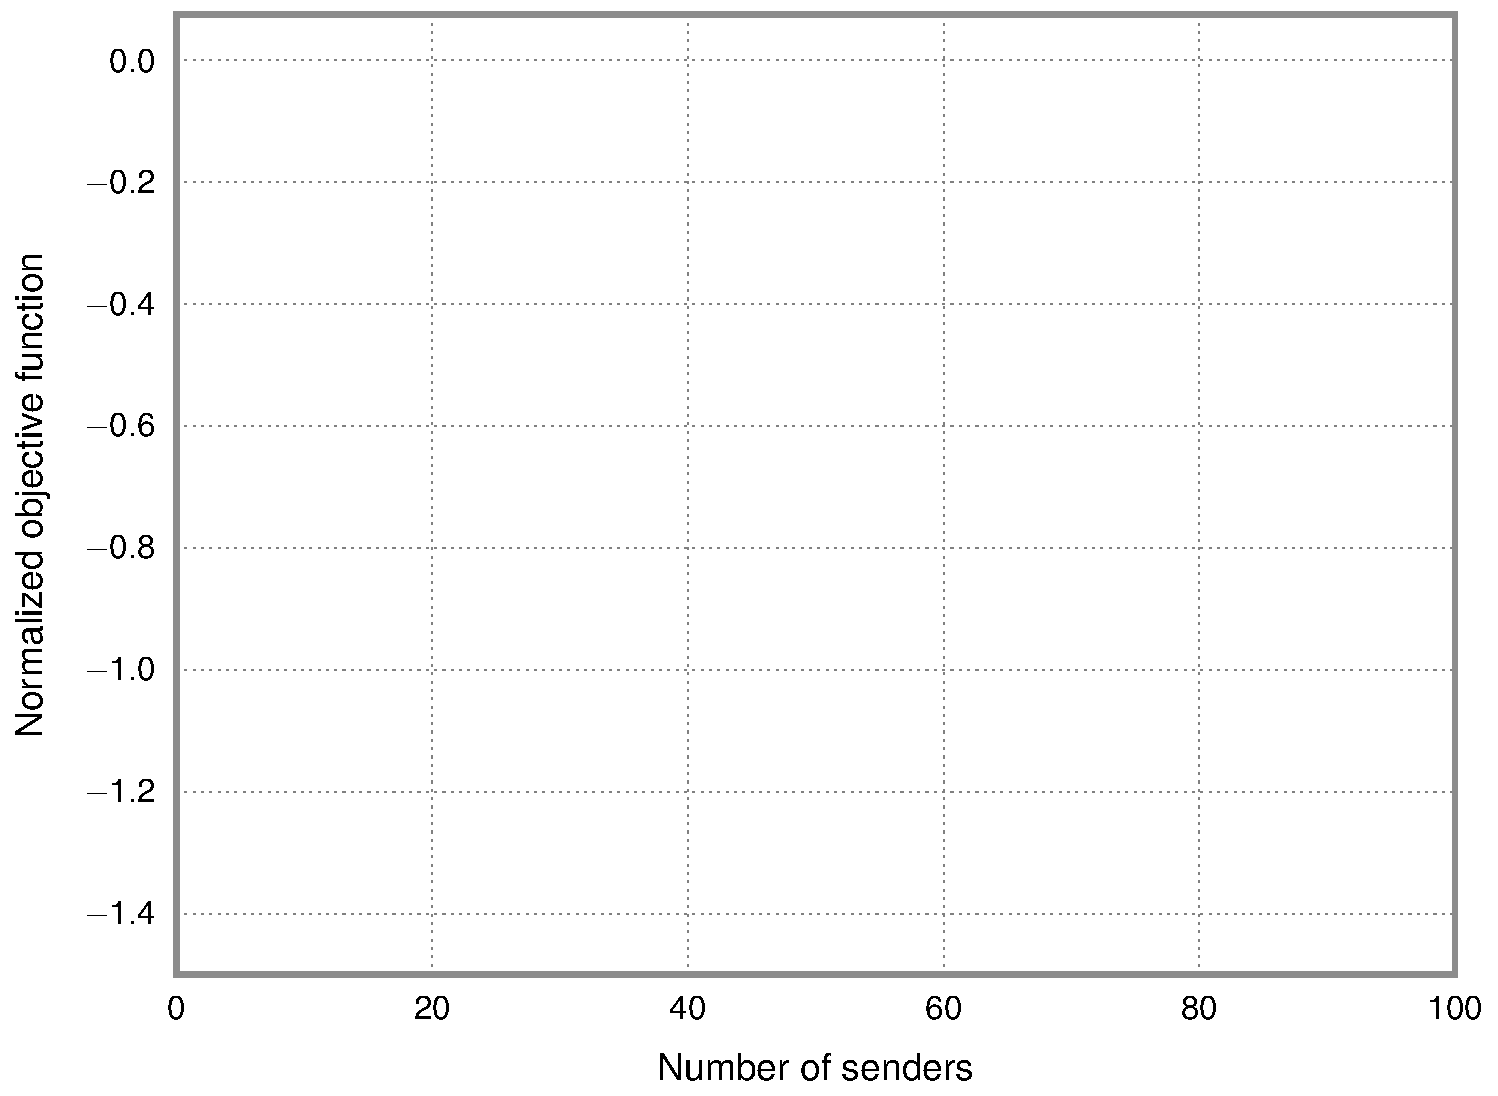
\includegraphics[width=3.1 in]{muxing-base.pdf}}\only<2>{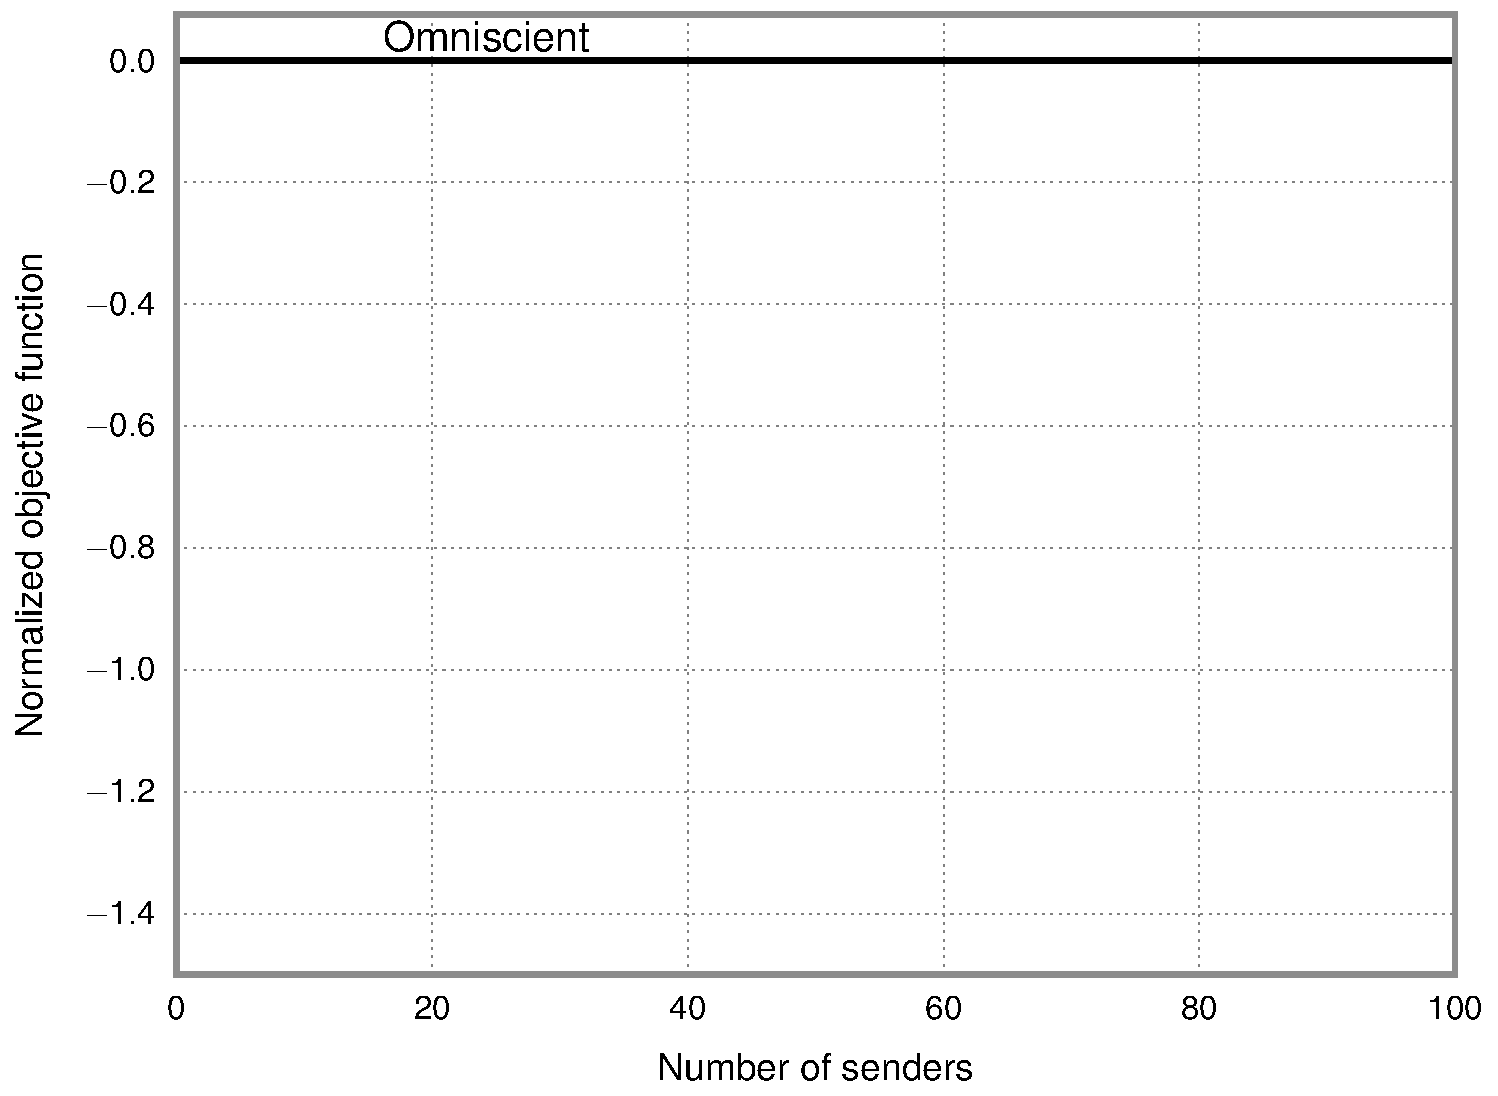
\includegraphics[width=3.1 in]{muxing-omniscient.pdf}}\only<3>{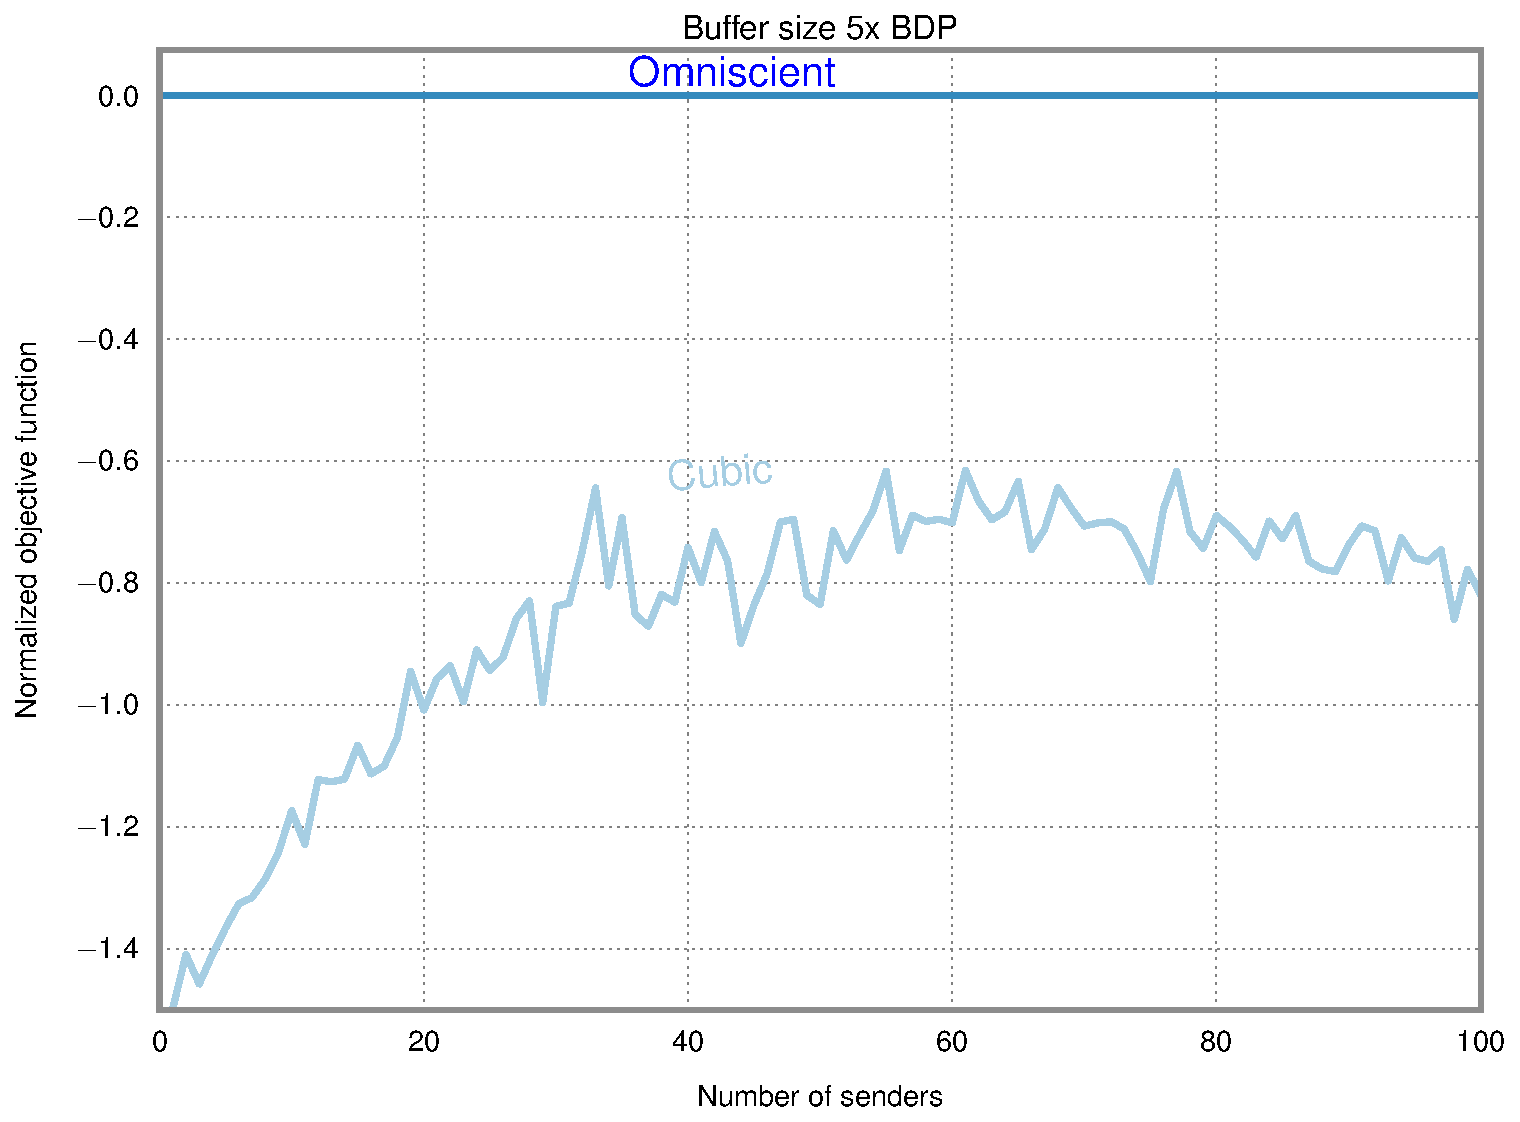
\includegraphics[width=3.1 in]{muxing-cubic.pdf}}\only<4>{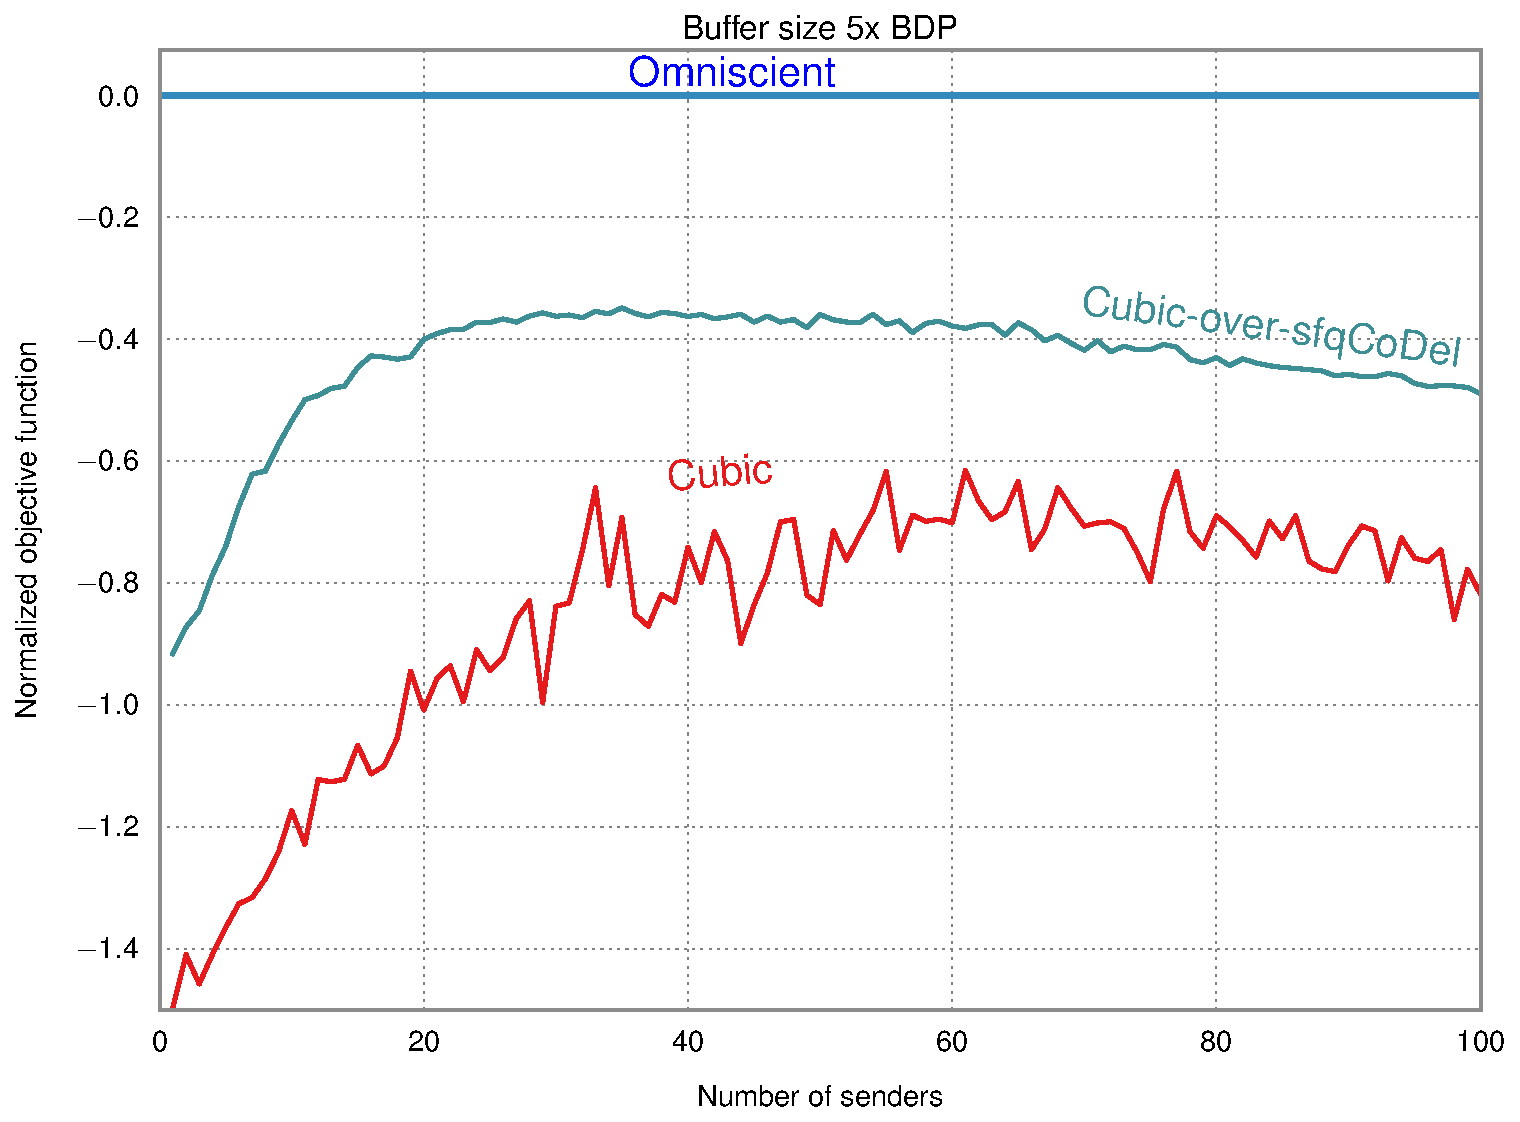
\includegraphics[width=3.1 in]{muxing-codel.pdf}}\only<5>{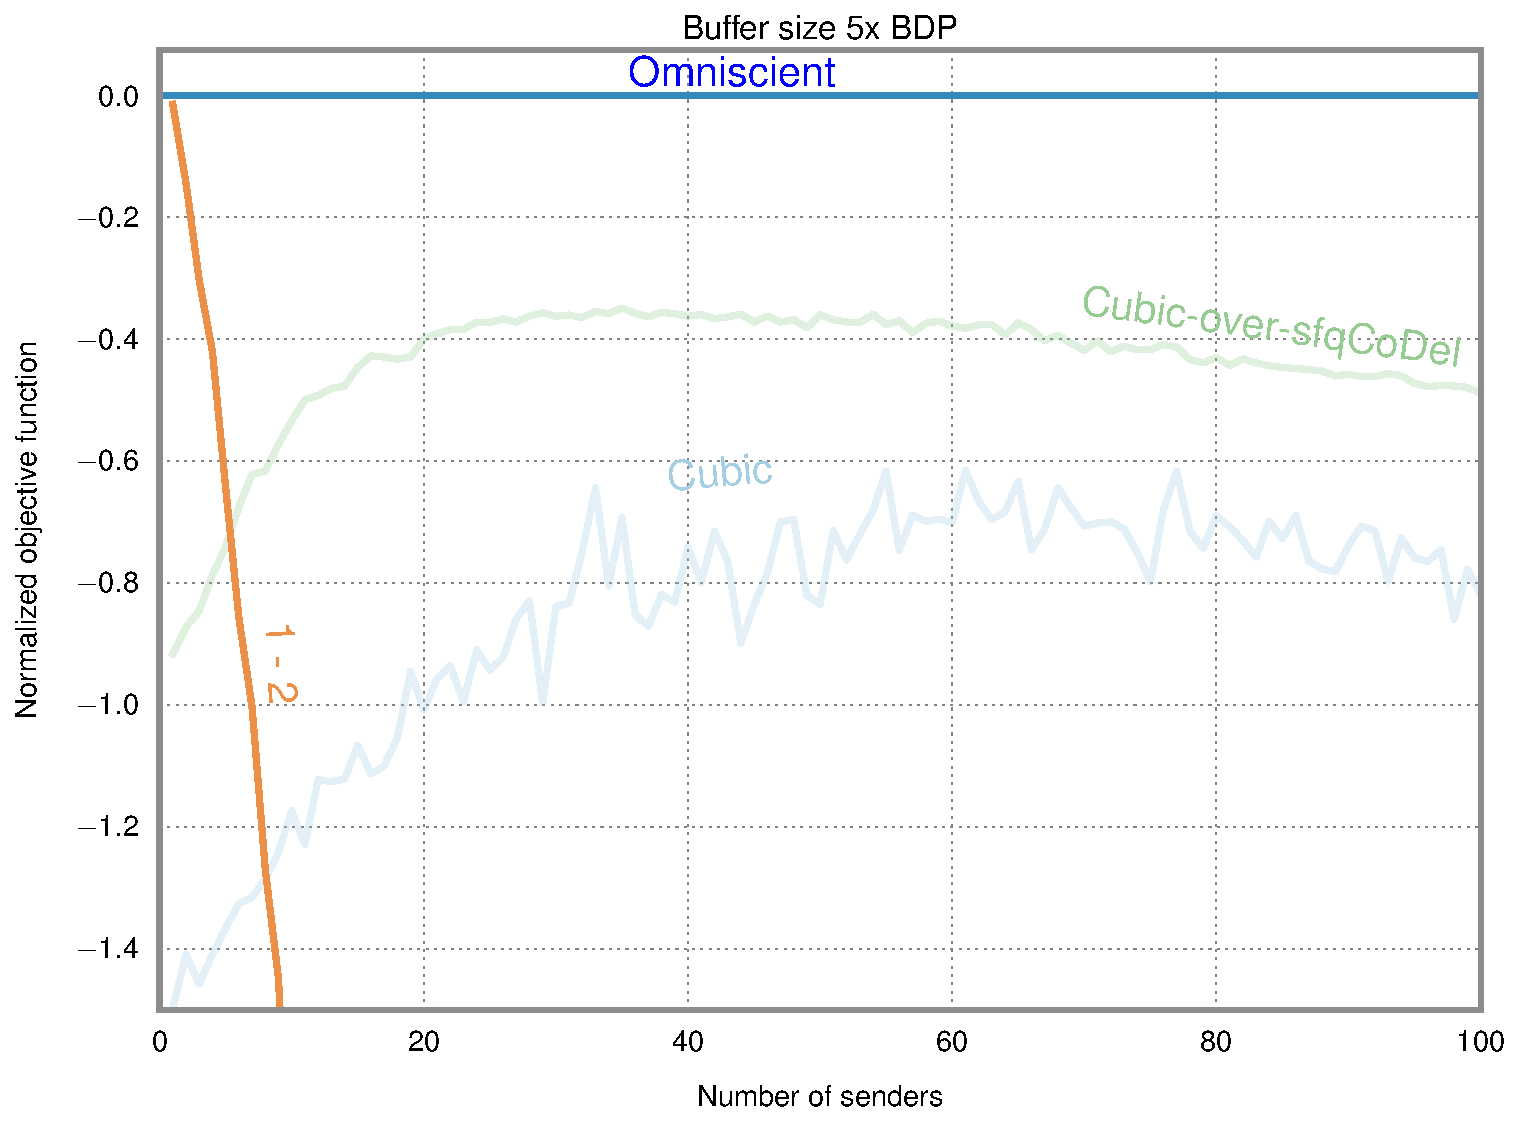
\includegraphics[width=3.1 in]{muxing-2.pdf}}\only<6>{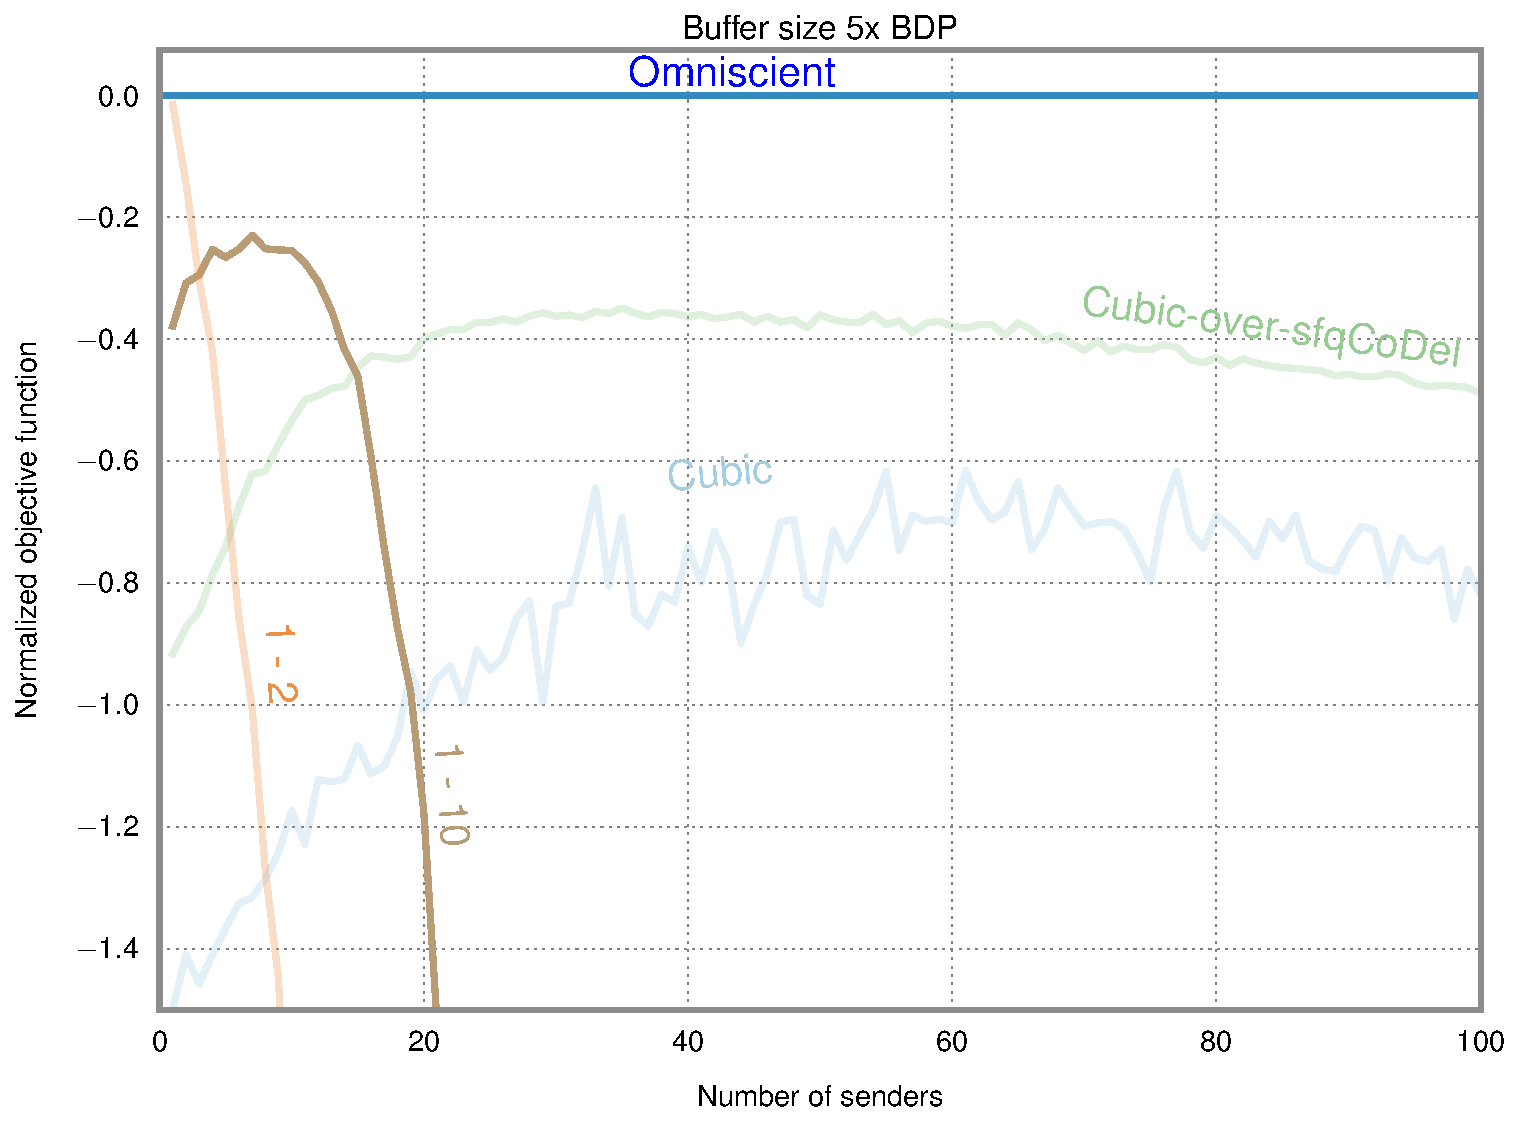
\includegraphics[width=3.1 in]{muxing-10.pdf}}\only<7>{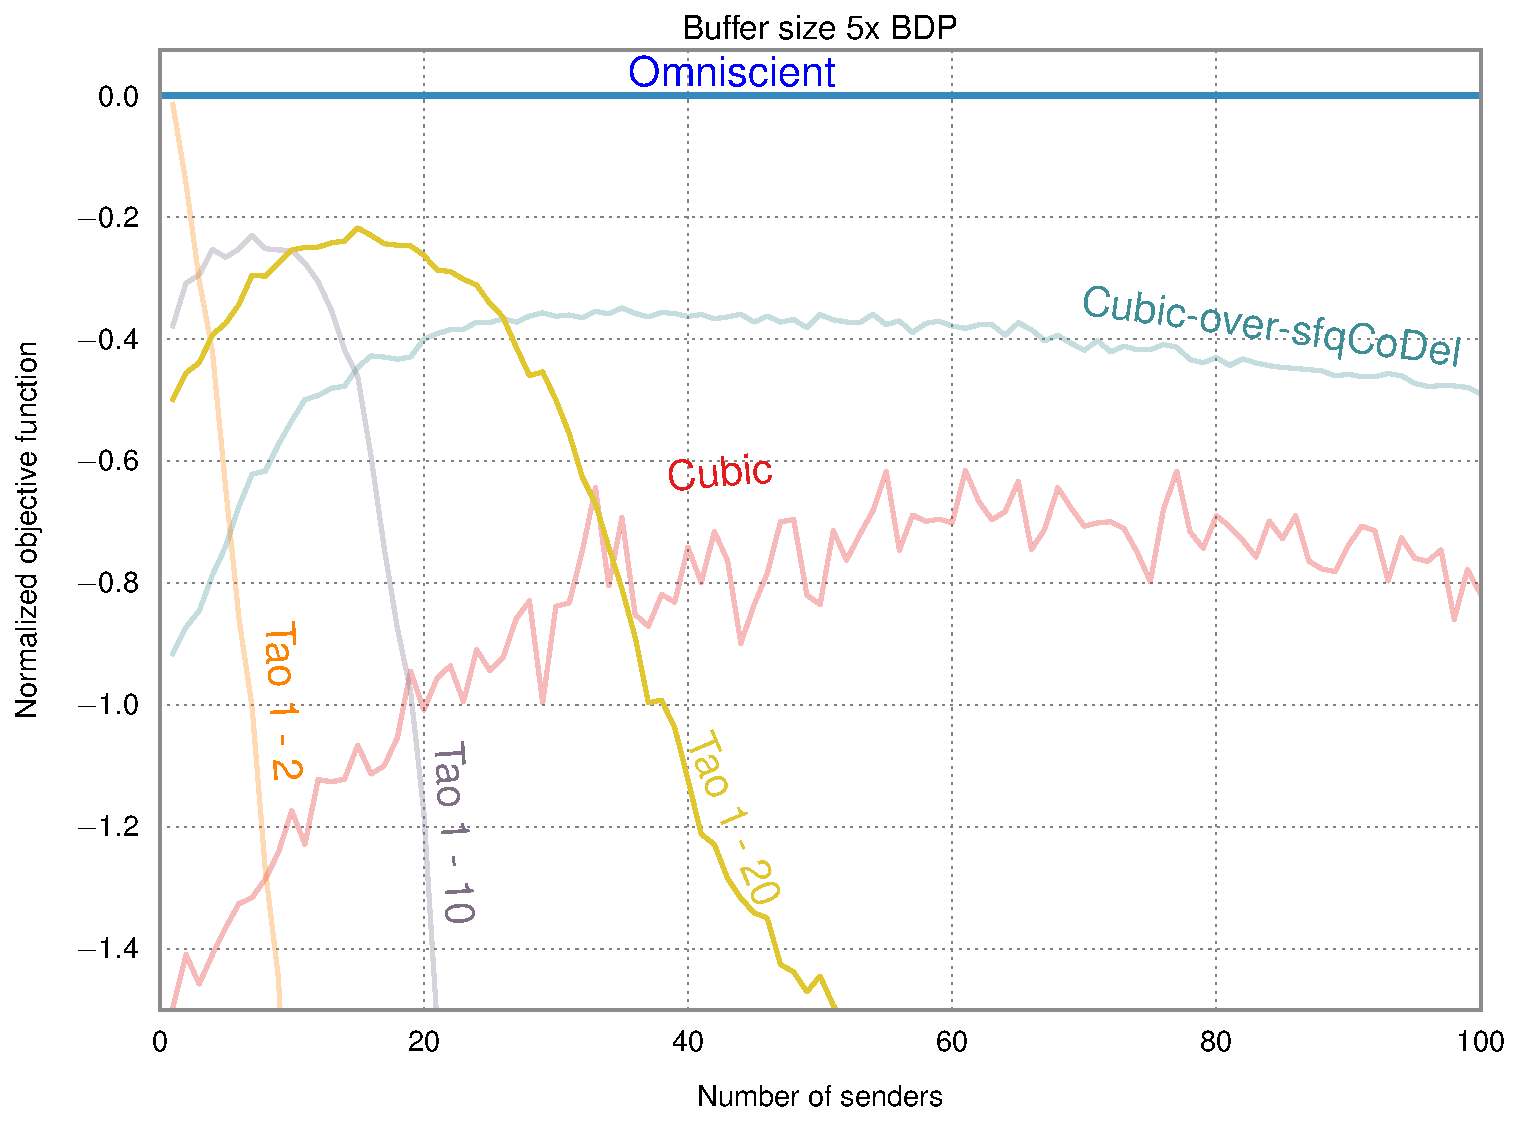
\includegraphics[width=3.1 in]{muxing-20.pdf}}\only<8>{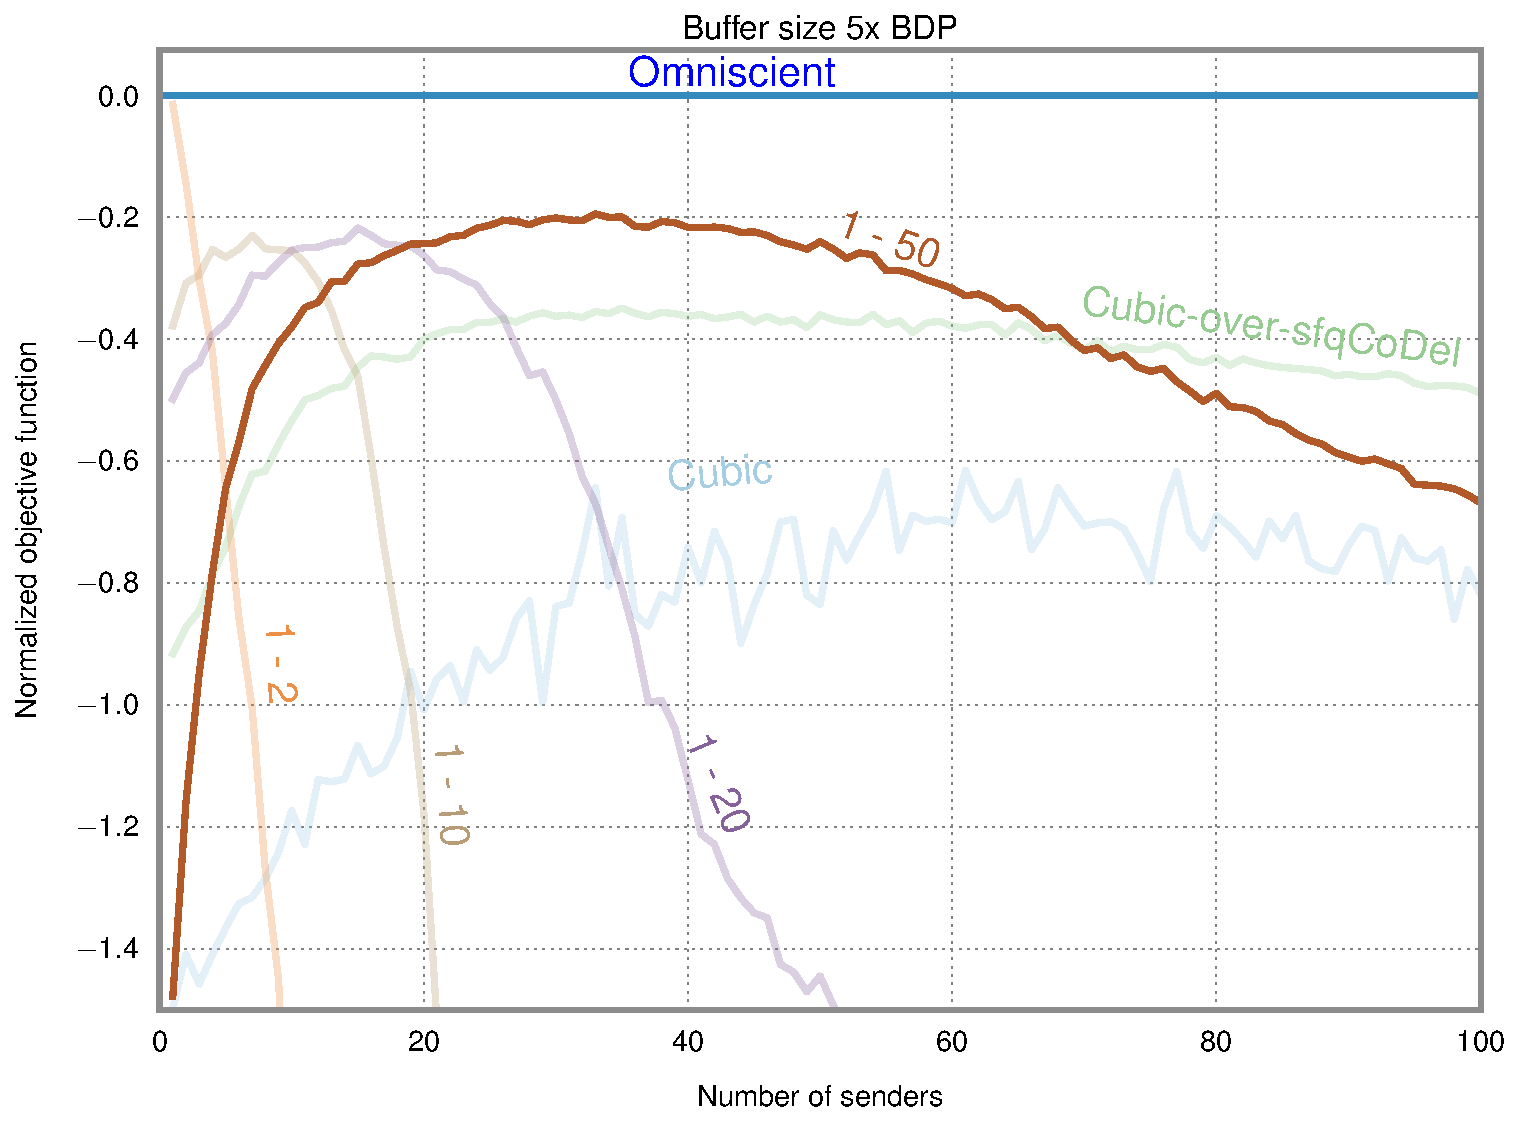
\includegraphics[width=3.1 in]{muxing-50.pdf}}\only<9>{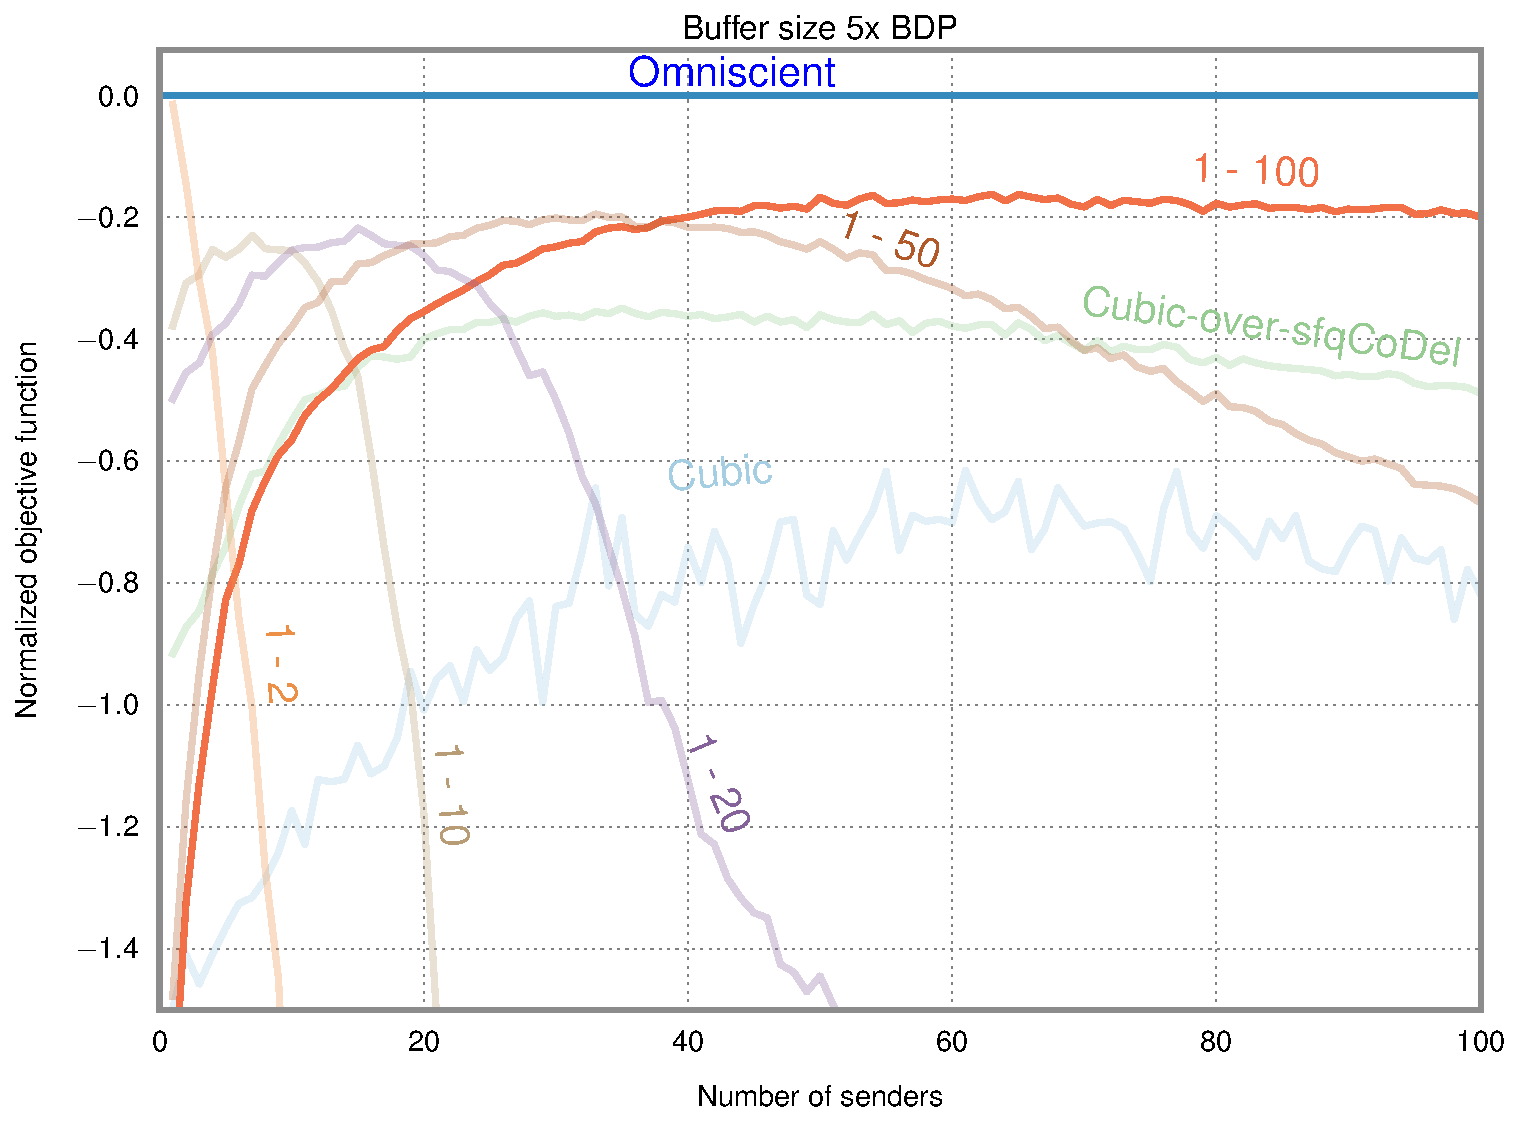
\includegraphics[width=3.1 in]{muxing-100.pdf}}

\only<10>{There is a tradeoff between performance at low and high degrees of multiplexing}

\end{centering}
\end{frame}
